\begin{enumerate}[label=\thesubsection.\arabic*, ref=\thesubsection.\theenumi]
	\item 
How many 3-digit numbers can be formed using three distinct single digit prime numbers?
\hfill (GATE~AE~2026)
\begin{enumerate}
    \item $64$
    \item $24$
    \item $12$
    \item $4$
\end{enumerate} 
\solution
 There are 4 	single digit prime numbers: 2,3,5 and 7. The desired numbers are given by
 \begin{align}
	 \perm{4}{3} = \frac{4!}{1!} = 24
 \end{align}


\item
In a group of students, 10 students like Mathematics, 12 students like English, 4 students like both Mathematics and English, and 6 students like neither Mathematics nor English. The number of students in the group is \underline{\hspace{1cm}}.
\hfill (GATE~AE~2026)
\begin{enumerate}
    \item $18$
    \item $20$
    \item $24$
    \item $32$
\end{enumerate} 

\solution 
Let $N$ be the total number of students in the group. If one student is chosen uniformly at random from the group, we define:
\begin{itemize}
    \item $M$: The event that the student likes Mathematics.
    \item $E$: The event that the student likes English.
\end{itemize}

The respective probabilities are expressed as:
\begin{align}
P\brak{M} &= \frac{10}{N}, \quad P\brak{E} = \frac{12}{N}
\end{align}
\begin{align}
P\brak{ME} = \frac{4}{N} \quad \text{(student likes both)}
\end{align}
\begin{align}
P\brak{\brak{M+E}'} = \frac{6}{N} \quad \text{(student likes neither)}
\end{align}

Since the total probability of the sample space is $1$:
\begin{align}
P\brak{M \cup E} + P\brak{\brak{M+E}'} = 1
\end{align}

From \eqref{eq:addition_theorem_probability}
\begin{align}
P\brak{M} + P\brak{E} - P\brak{ME} + P\brak{\brak{M+E}'} = 1
\end{align}

Substitute the probabilities in terms of $N$:
\begin{align}
\frac{10}{N} + \frac{12}{N} - \frac{4}{N} + \frac{6}{N} = 1
\end{align}

\begin{align}
\frac{10 + 12 - 4 + 6}{N} = 1
\end{align}
\begin{align}
\frac{24}{N} = 1 \implies N = 24
\end{align}

\item 
Given a square of side $s=4\text{cm}$ and two circles, one with known radius $r_1=1\text{cm}$ and another with unknown radius $r_2$, such that both of them touch each other externally and also the square, find the value of $r_2$. Also describe how the figure in the problem can be constructed. \hfill (GATE~AE~2026)
\begin{figure}[H]
\begin{center}
\begin{tikzpicture}[scale=1.5, >=Stealth]
    \pgfmathsetmacro{\side}{4.0}
    \pgfmathsetmacro{\rone}{1.0}
    \pgfmathsetmacro{\rtwo}{7 - 4*sqrt(2)}

    \coordinate (W) at (0, 0);
    \coordinate (X) at (\side, 0);
    \coordinate (Y) at (\side, \side);
    \coordinate (V) at (0, \side);

    \draw[thick] (W) -- (X) -- (Y) -- (V) -- cycle;

    \draw[thick] (\side-0.25, \side) -- (\side-0.25, \side-0.25) -- (\side, \side-0.25);
    \draw[thick] (\side-0.25, 0) -- (\side-0.25, 0.25) -- (\side, 0.25);

    \coordinate (O1) at (\rone, \rone);
    \coordinate (O2) at (\side-\rtwo, \side-\rtwo);

    \coordinate (P) at (0, \rone);
    \coordinate (Q) at (\rone, 0);
    \coordinate (S) at (\side-\rtwo, \side);
    \coordinate (R) at (\side, \side-\rtwo);

    \pgfmathsetmacro{\Tx}{\rone + \rone*cos(45)}
    \pgfmathsetmacro{\Ty}{\rone + \rone*sin(45)}
    \coordinate (T) at (\Tx, \Ty);

    \draw[thick] (O1) circle (\rone);
    \draw[thick] (O2) circle (\rtwo);

    \draw[dotted, thick, ->] (O1) -- (2*\rone, \rone) 
        node[midway, above=-1pt] {\small $r_1 = 1\text{ cm}$};

    \draw[dotted, thick, ->] (O2) -- (\side-2*\rtwo, \side-\rtwo) 
        node[midway, above=-1pt] {\small $r_2$};

    \node[left=2pt] at (V) {$V$};
    \node[left=2pt] at (W) {$W$};
    \node[right=2pt] at (X) {$X$};
    \node[right=2pt] at (Y) {$Y$};

    \node[left=2pt] at (P) {$P$};
    \node[below=2pt] at (Q) {$Q$};
    \node[above=2pt] at (S) {$S$};
    \node[right=2pt] at (R) {$R$};
    \node[below left=1pt] at (T) {$T$};

    \node[below left=1pt] at (O1) {$O_1$};
    \node[below right=1pt] at (O2) {$O_2$};

    \node[below right] at (1.6, 0.3) {$C_1$};
    \node[below right] at (\side-0.5, \side-1.5) {$C_2$};

    \draw[dotted, thick, <->] (0, \side+0.5) -- (\side, \side+0.5) 
        node[midway, fill=white, inner sep=2pt] {\small $\overline{VY} = 4\text{ cm}$};

    \draw[dotted, thick, <->] (-0.5, 0) -- (-0.5, \side) 
        node[midway, fill=white, inner sep=2pt, rotate=90] {\small $\overline{VW} = 4\text{ cm}$};

\end{tikzpicture}

\makeatletter
    \long\def\@makecaption#1#2{%
      \vskip\abovecaptionskip
      \begin{center}
        #1 #2
      \end{center}
      \vskip\belowcaptionskip}
\caption{Touching Circles and Square}
    \label{fig:2}
\end{center}
\end{figure}
\solution
\begin{enumerate}
\item Solving for $r_2$
Let the side of the square be $s$, radius of the first circle be $r_1$ and that of the unknown circle be $r_2$. Clearly from figure:
     \begin{align}
      WO_1+ O_1T+ TO_2 +O_2Y= \sqrt{2}s 
     \end{align}
     We know that:
     \begin{align}
     WO_1= \sqrt{2}r_1,    O_1T = r_1, TO_2 = r_2 , O_2W = \sqrt{2}r_2. 
     \end{align}
     Substituting this in our result from point (4.2) we get:
     \begin{align}
     r_2 = \frac{\sqrt{2}s - \brak{\sqrt{2} + 1}r_1}{\sqrt{2} + 1}.
     \end{align}  
     Substituting the values of $s$ and $r_1$, we get:
     \begin{align}
	     r_2 = \brak{7-4\sqrt{2}}\text{cm} 
     \end{align}
\item \textbf{General method for construction:}

Vertices of the square:
\begin{align}
\vec{W} = \myvec{0\\0}, \quad \vec{X} = \myvec{s\\0}, \quad \vec{Y} = \myvec{s\\s}, \quad \vec{V} = \myvec{0\\s}
\end{align}
Circle $C_1$ ($r_1$):
\begin{align}
\vec{O}_1 = \myvec{r_1\\r_1}, \quad \vec{P} = \myvec{0\\r_1}, \quad \vec{Q} = \myvec{r_1\\0}
\end{align}
Circle $C_2$ ($r_2$):
\begin{align}
\vec{O}_2 = \myvec{s-r_2\\s-r_2}, \quad \vec{S} = \myvec{s-r_2\\s}, \quad \vec{R} = \myvec{s\\s-r_2}
\end{align}
Line of centers and contact point $\vec{T}$:
\begin{align}
\vec{O}_2 - \vec{O}_1 = \myvec{s-r_2-r_1\\s-r_2-r_1} = (s-r_2-r_1)\myvec{1\\1}
\end{align}
Now, given that the circles are touching, we know that:
\begin{align}
	\frac{O_1T}{O_2T} = \frac{r_1}{r_2}
\end{align}
\begin{align}
\frac{O_1T}{O_1O_2} = \frac{r_1}{r_1+r_2}
\end{align}
Hence, using the equation of line of centers obtained, we have:
\begin{align}
\vec{T} = \vec{O}_1 + \frac{r_1}{r_1+r_2}(\vec{O}_2 - \vec{O}_1)
\end{align}
\begin{lstlisting}[frame=single, basicstyle=\rmfamily, escapeinside={(*@}{@*)}]
(*@\makebox[\dimexpr\linewidth-2\fboxsep-2\fboxrule\relax][c]{codes/Circle.py}@*)
\end{lstlisting}
\begin{figure}[H]
    \centering
    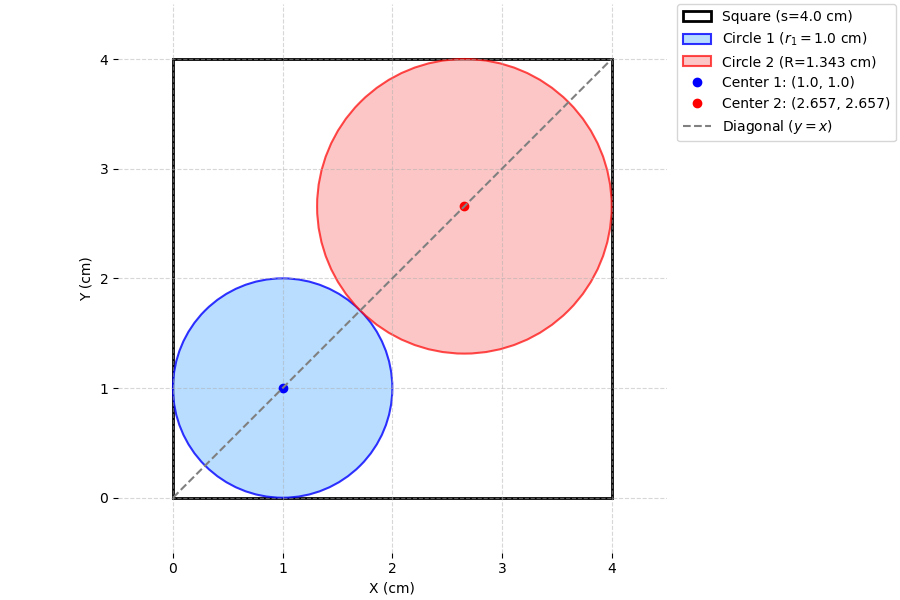
\includegraphics[width=0.75\linewidth]{figs/Circle.png}
	\makeatletter
    \long\def\@makecaption#1#2{%
      \vskip\abovecaptionskip
      \begin{center}
        #1 #2
      \end{center}
      \vskip\belowcaptionskip}
    \makeatother
    \caption{Square with Tangent Circles}
    \label{fig:3}
\end{figure}
\end{enumerate}


\item Consider the contour $C$ shown in the figure below. For the vector $\vec{F} = \brak{x + 2y}\hat{e}_x + \brak{2x + 4y}\hat{e}_y$, the integral $\oint_{C} \vec{F} \cdot d\vec{l} = \underline{\hspace{2cm}}$.

Here $d\vec{l}$ represents an infinitesimal length along the contour $C$.\hfill (GATE~AE~2026)
\begin{enumerate}
    \item $0$
    \item $2$
    \item $4$
    \item $6$
\end{enumerate} 

\begin{figure}[H]
\begin{center}
\begin{tikzpicture}[scale=1.55, >=Stealth]
    \tikzset{
        segment arrow/.style={
            postaction={
                decorate,
                decoration={
                    markings,
                    mark=at position 0.55 with {\arrow[scale=1.2]{Stealth[length=6pt, width=5pt]}}
                }
            }
        }
    }

    \draw[thick, ->] (-2.2, 0) -- (2.2, 0) node[right] {$x$};
    \draw[thick, ->] (0, -0.8) -- (0, 2.6) node[left] {$y$};

    \coordinate (O) at (0, 0);
    \coordinate (P) at (1, 1);
    \coordinate (Q) at (0, 2);
    \coordinate (R) at (-1, 1);

    \draw[line width=1.5pt, segment arrow] (O) -- (P);
    \draw[line width=1.5pt, segment arrow] (P) -- (Q);
    \draw[line width=1.5pt, segment arrow] (Q) -- (R);
    \draw[line width=1.5pt, segment arrow] (R) -- (O);

    \node[below right=2pt] at (0.5, 0.5) {$C$};

    \node[below left=1pt] at (O) {$\mathbf{O}$};
    \node[below right=1pt] at (O) {$(0,0)$};

    \node[above right=1pt] at (P) {$\mathbf{P}$};
    \node[below right=1pt] at (P) {$(1,1)$};

    \node[above left=1pt] at (Q) {$\mathbf{Q}$};
    \node[above right=1pt] at (Q) {$(0,2)$};

    \node[above left=1pt] at (R) {$\mathbf{R}$};
    \node[below left=1pt] at (R) {$(-1,1)$};

\end{tikzpicture}


\makeatletter
    \long\def\@makecaption#1#2{%
      \vskip\abovecaptionskip
      \begin{center}
        #1 #2
      \end{center}
      \vskip\belowcaptionskip}
    \makeatother
   \caption{Contour C}
    \label{fig:4}
\end{center}
\end{figure}
\solution

We can break the closed path $C$ into its four straight line paths: $O \to P \to Q \to R \to O$.

\begin{align}
\mathbf{F} \cdot d\mathbf{l} = \myvec{x + 2y \\ 2x + 4y} \cdot \myvec{dx \\ dy}
\end{align}
\begin{align}
\mathbf{F}^T d\mathbf{l} = \myvec{x + 2y \\ 2x + 4y}^T \myvec{dx \\ dy} = \myvec{x + 2y & 2x + 4y} \myvec{dx \\ dy}
\end{align}
\begin{align}
= \myvec{(x + 2y)dx + (2x + 4y)dy}
\end{align}
The general line integral expression to evaluate along any path is:
\begin{align}
\mathbf{I} = \int \brak{x + 2y}\,dx + \brak{2x + 4y}\,dy
\end{align}
Path $O\brak{0,0} \to P\brak{1,1}$
\begin{itemize}
    \item Equation of line: $y = x \implies dy = dx$
    \item Limits: $x$ goes from $0$ to $1$
\end{itemize}
\begin{align}
\mathbf{I_1} = \int_0^1 \brak{x + 2x}\,dx + \brak{2x + 4x}\,dx = \int_0^1 9x\,dx = \left[ \frac{9x^2}{2} \right]_0^1 = \frac{9}{2}
\end{align}

Path $P\brak{1,1} \to Q\brak{0,2}$
\begin{itemize}
    \item Equation of line: $y = 2 - x \implies dy = -dx$
    \item Limits: $x$ goes from $1$ to $0$
\end{itemize}
\begin{align}
\mathbf{I_2} = \int_1^0 \brak{x + 2\brak{2-x}}\,dx + \brak{2x + 4\brak{2-x}}\brak{-dx}
\end{align}
\begin{align}
\mathbf{I_2} = \int_1^0 \left[ \brak{4-x} - \brak{8-2x} \right]\,dx = \int_1^0 \brak{x-4}\,dx = \left[ \frac{x^2}{2} - 4x \right]_1^0 = \frac{7}{2}
\end{align}

Path $Q\brak{0,2} \to R\brak{-1,1}$
\begin{itemize}
    \item Equation of line: $y = x + 2 \implies dy = dx$
    \item Limits: $x$ goes from $0$ to $-1$
\end{itemize}
\begin{align}
\mathbf{I_3} = \int_0^{-1} \brak{x + 2\brak{x+2}}\,dx + \brak{2x + 4\brak{x+2}}\,dx = \int_0^{-1} \brak{9x + 12}\,dx
\end{align}
\begin{align}
\mathbf{I_3} = \left[ \frac{9x^2}{2} + 12x \right]_0^{-1} = \brak{\frac{9}{2} - 12} - 0 = -\frac{15}{2}
\end{align}

Path $R\brak{-1,1} \to O\brak{0,0}$
\begin{itemize}
    \item Equation of line: $y = -x \implies dy = -dx$
    \item Limits: $x$ goes from $-1$ to $0$
\end{itemize}
\begin{align}
\mathbf{I_4} = \int_{-1}^0 \brak{x + 2\brak{-x}}\,dx + \brak{2x + 4\brak{-x}}\brak{-dx} = \int_{-1}^0 x\,dx
\end{align}
\begin{align}
\mathbf{I_4} = \left[ \frac{x^2}{2} \right]_{-1}^0 = 0 - \frac{1}{2} = -\frac{1}{2}
\end{align}

Summing the integrals across all four line segments:
\begin{align}
\mathbf{I = I_1 + I_2 + I_3 + I_4}
\end{align}
\begin{align}
\mathbf{I} = \frac{9}{2} + \frac{7}{2} - \frac{15}{2} - \frac{1}{2} = \frac{16 - 16}{2} = 0
\end{align}\\
\begin{lstlisting}[frame=single, basicstyle=\rmfamily, escapeinside={(*@}{@*)}]
(*@\makebox[\dimexpr\linewidth-2\fboxsep-2\fboxrule\relax][c]{codes/Line\_Integral.py}@*)
\end{lstlisting}
\begin{figure}[H]
    \centering
    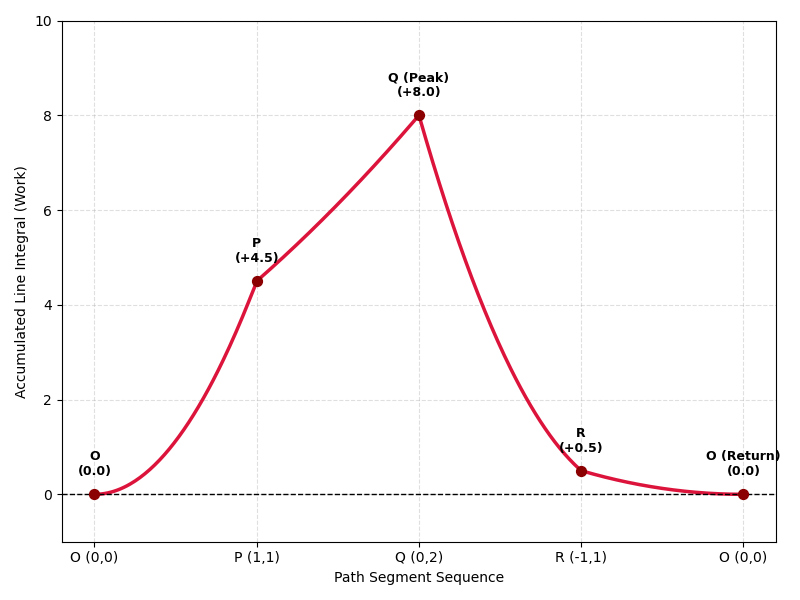
\includegraphics[width=0.75\linewidth]{figs/Line_Integral.png}
	\makeatletter
    \long\def\@makecaption#1#2{%
      \vskip\abovecaptionskip
      \begin{center}
        #1 #2
      \end{center}
      \vskip\belowcaptionskip}
    \makeatother
    \caption{Visualising the Cancellation of Integrals}
    \label{fig:5}
\end{figure}
\item

The Fourier series representation of a square wave is shown in the figure below. The fluctuations seen near $x = \pm 1$ are named after which one of the following scientists? \hfill(GATE~AE~2026)

\begin{enumerate}
    \item Cauchy
    \item Fourier
    \item Gibbs
    \item Laplace
\end{enumerate}
\begin{figure}[H]
    \centering
	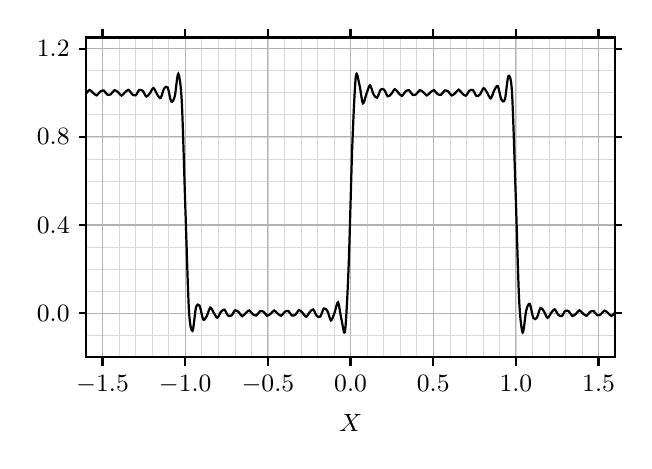
\begin{tikzpicture}[x=2.1cm, y=2.8cm]
        % Background Grid
        \draw[gray!30, line width=0.2pt, step=0.1] (-1.6,-0.2) grid (1.6,1.25);
        \draw[gray!60, line width=0.4pt, xstep=0.5, ystep=0.4] (-1.6,-0.2) grid (1.6,1.25);

        % Outer Bounding Box
        \draw[thick] (-1.6,-0.2) rectangle (1.6,1.25);

        % X-Axis Ticks & Labels
        \foreach \x in {-1.5, -1.0, -0.5, 0.0, 0.5, 1.0, 1.5} {
            \draw[thick] (\x,-0.2) -- (\x,-0.24);
            \draw[thick] (\x,1.25) -- (\x,1.29);
            \node[below, font=\small] at (\x,-0.24) {\pgfmathprintnumber[fixed,precision=1,zerofill]{\x}};
        }

        % Y-Axis Ticks & Labels
        \foreach \y in {0.0, 0.4, 0.8, 1.2} {
            \draw[thick] (-1.6,\y) -- (-1.64,\y);
            \draw[thick] (1.6,\y) -- (1.64,\y);
            \node[left, font=\small] at (-1.64,\y) {\pgfmathprintnumber[fixed,precision=1,zerofill]{\y}};
        }

        % Axis Label
        \node[below=14pt, font=\small] at (0,-0.24) {$X$};

        % Fourier Square Wave Plot
        \draw[thick, black, declare function={
            f(\x) = 0.5 + (2/pi)*(
                sin(deg(pi*\x)) 
                + (1/3)*sin(deg(3*pi*\x)) 
                + (1/5)*sin(deg(5*pi*\x)) 
                + (1/7)*sin(deg(7*pi*\x)) 
                + (1/9)*sin(deg(9*pi*\x)) 
                + (1/11)*sin(deg(11*pi*\x)) 
                + (1/13)*sin(deg(13*pi*\x)) 
                + (1/15)*sin(deg(15*pi*\x)) 
                + (1/17)*sin(deg(17*pi*\x)) 
                + (1/19)*sin(deg(19*pi*\x)) 
                + (1/21)*sin(deg(21*pi*\x)) 
                + (1/23)*sin(deg(23*pi*\x)) 
                + (1/25)*sin(deg(25*pi*\x))
            );
        }] 
        plot[domain=-1.6:1.6, samples=150, smooth] (\x, {f(\x)});
    \end{tikzpicture}


    	\makeatletter
    \long\def\@makecaption#1#2{%
      \vskip\abovecaptionskip
      \begin{center}
        #1 #2
      \end{center}
      \vskip\belowcaptionskip}
    \makeatother
    \caption{Fourier Square Wave Representation}
    \label{fig:6}
\end{figure}
\solution
\begin{enumerate}
\item Gibbs Phenomenon
\begin{itemize}
	\item Explanation of Gibbs Phenomenon: Every periodic function can be expressed as a sum of sines and cosines. Gibbs phenomenon is the overshoot and high-frequency oscillation ("ringing") that occurs when approximating a function with jump discontinuities using a finite (truncated) Fourier series. Even as the number of terms $N$ approaches infinity, the overshoot near the jump discontinuity does not vanish; instead, it narrows in width while maintaining a fixed percentage height relative to the size of the jump.
	\item Reason: When approximating a step function or square wave, Fourier series synthesize the shape using smooth, continuous sinusoids ($\sin$ and $\cos$). Because continuous functions cannot instantaneously step from one value to another, the Fourier series overcompensates near the vertical edge.
\end{itemize}
\item Finding the fourier coefficients for a square wave 
We will use the result \eqref{eq:Fourier_1}. Considering $f_0 = \frac{1}{4}$, $T_0 = 4$, and the integration interval $\brak{-\frac{1}{2f_0}, \frac{1}{2f_0}} = \brak{-2, 2}$:
\begin{align}
c_k &= \frac{1}{4} \int_{-1}^{1} e^{-j \frac{\pi k t}{2}} \, dt
\end{align}
\begin{align}
c_k = 
\begin{dcases}
    \frac{1}{4} \int_{-1}^{1} 1 \, dt = \frac{1}{2}, & k = 0 \\[12pt]
    \frac{1}{4} \left[ \frac{e^{-j \frac{\pi k t}{2}}}{-j \frac{\pi k}{2}} \right]_{-1}^{1} = \frac{1}{2} \sinc\brak{\frac{\pi k}{2}}, & k \neq 0
\end{dcases}
\end{align}
\begin{lstlisting}[frame=single, basicstyle=\rmfamily, escapeinside={(*@}{@*)}]
(*@\makebox[\dimexpr\linewidth-2\fboxsep-2\fboxrule\relax][c]{codes/Fourier.py}@*)
\end{lstlisting}
\begin{figure}[H]
    \centering
    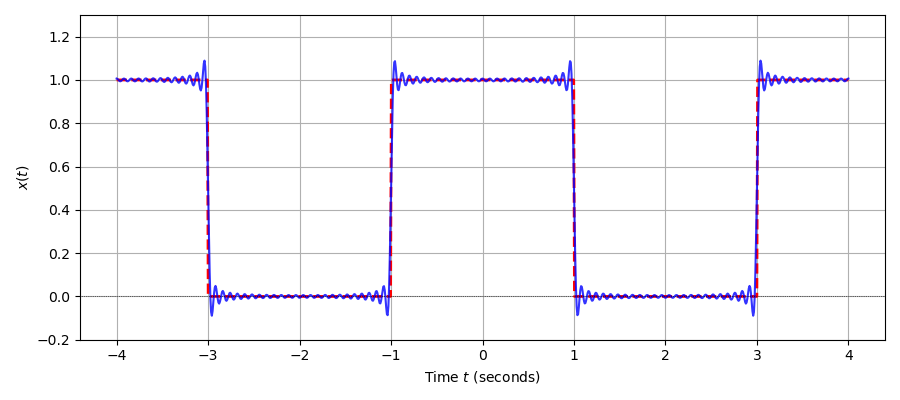
\includegraphics[width=0.75\linewidth]{figs/Fourier.png}
	\makeatletter
    \long\def\@makecaption#1#2{%
      \vskip\abovecaptionskip
      \begin{center}
        #1 #2
      \end{center}
      \vskip\belowcaptionskip}
    \makeatother
    \caption{Plot Generated}
    \label{fig:7}
\end{figure}

\end{enumerate}
\item If a matrix can be written as $\mathbf{A} = \mathbf{uv^T}$, where both $u$ and $v$ are $n$-dimensional real-valued non-zero column vectors, then the rank of the matrix $\mathbf{A}$ is \underline{\hspace{1cm}}.
\hfill (GATE~AE~2026)

\solution 

We will solve the above problem with an example. Consider $3$-dimensional non-zero vectors $\mathbf{u} = \myvec{1 \\ 2 \\ 3}$ and $\mathbf{v} = \myvec{1 \\ 4 \\ 2}$.

The matrix $\mathbf{A}$ is formed as:
\begin{align}
\mathbf{A} = \mathbf{uv^T} &= \myvec{1 \\ 2 \\ 3} \myvec{1 & 4 & 2} \\
&= \myvec{
1 & 4 & 2 \\
2 & 8 & 4 \\
3 & 12 & 6
}
\end{align}

Applying elementary row transformations step-by-step:

Eliminate the non-zero entry in the second row using $R_2 \to R_2 - 2R_1$:
\begin{align}
\mathbf{A} \xrightarrow{R_2 \to R_2 - 2R_1} \myvec{
1 & 4 & 2 \\
0 & 0 & 0 \\
3 & 12 & 6
}
\end{align}

Eliminate the non-zero entry in the third row using $R_3 \to R_3 - 3R_1$:
\begin{align}
\xrightarrow{R_3 \to R_3 - 3R_1} \myvec{
1 & 4 & 2 \\
0 & 0 & 0 \\
0 & 0 & 0
}
\end{align}
The matrix is now in row echelon form with only $1$ non-zero row. Hence, $\text{rank}\brak{\mathbf{A}} = 1$.

\item
An $n \times n$ square matrix $\mathbf{A}$ satisfies $\mathbf{A^T} = \mathbf{A^{-1}}$. The determinant of this matrix may take which of the following value(s)? \hfill (GATE~AE~2026)
\begin{enumerate}
	\item $1$
	\item $-1$
	\item $n$
	\item $0$
\end{enumerate}

\solution 
We are given that matrix $A$ satisfies:
\begin{align}
\mathbf{A^T = A^{-1}}
\end{align}

Taking the determinant of both sides of the given matrix equation:
\begin{align}
\mydet{\mathbf{A^T}} = \mydet{\mathbf{A^{-1}}}
\end{align}

Using \eqref{eq:Matrices_1}:
\begin{align}
         \mydet{\mathbf{A^T}} = \mydet{\mathbf{A}}
\end{align}
\begin{align}
        \mydet{\mathbf{A^{-1}}} = \frac{1}{\mydet{\mathbf{A}}}
    \end{align} 

Replacing both sides using the above properties gives:
\begin{align}
\mydet{\mathbf{A}} = \frac{1}{\mydet{\mathbf{A}}}
\end{align}

Multiplying both sides by $\mydet{\mathbf{A}}$:
 \begin{align}
\brak{\mydet{\mathbf{A}}}^2 = 1 \implies \mydet{\mathbf{A}} = \pm 1
\end{align} 

\item
	
Given the velocity and position vectors of a satellite along with its gravitational parameter $\mu=GM$, determine the trajectory of the satellite. \hfill (GATE AE 2026) 
\begin{enumerate}
    \item Circle
    \item Hyperbola
    \item Parabola
    \item Straight Line
\end{enumerate} 

Position vector: 
    \begin{align}
    \vec{r} = 8000\hat{p} + 9000\hat{q} \text{ km}
    \end{align}
Velocity vector:
    \begin{align}
    \vec{v} = -6\hat{p} + 6\hat{q} \text{ km/s}
    \end{align}
Gravitational parameter: 
    \begin{align}
    \mu = 398600 \text{ km}^3/\text{s}^2
    \end{align}

\solution 
We are given :
\begin{align}
	\vec{r}=\myvec{8000\\9000}, \vec{v}=\myvec{-6\\6}
\end{align}
From \eqref{eq:Gravitation_1}, Specific Angular Momentum \brak{h_0}:
\begin{align}
= |8000\brak{6} - 9000\brak{-6}| = 102000 \text{ km}^2/\text{s}
\end{align}

From \eqref{eq:Gravitation_2}, eccentricity squared \brak{e^2}:
\begin{align}
= 1 + \frac{2\brak{2.898}\brak{102000}^2}{\brak{398600}^2} \approx 1 + 0.3795 = 1.3795
\end{align}
From \eqref{eq:Gravitation_3}, we have:
\begin{align}
\mydet{\mathbf{V}}=1-1.3795=-0.3795
\end{align}
From \ref{item:Hyperbola}, we can conclude that the trajectory of the satellite is a Hyperbola.

\begin{lstlisting}[frame=single, basicstyle=\rmfamily, escapeinside={(*@}{@*)}]
(*@\makebox[\dimexpr\linewidth-2\fboxsep-2\fboxrule\relax][c]{codes/Satellite.py}@*)
\end{lstlisting}
\begin{figure}[H]
    \centering
    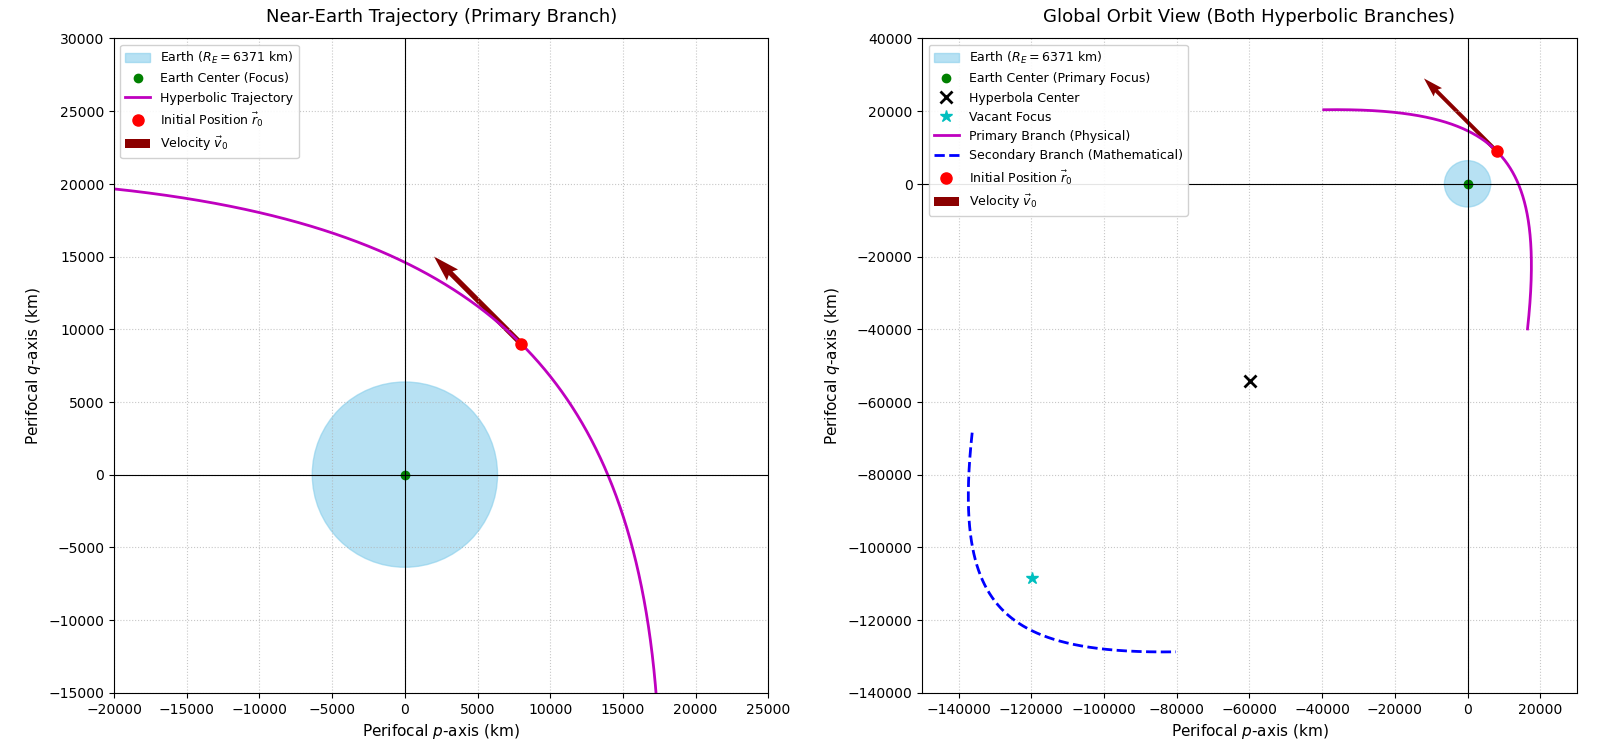
\includegraphics[width=1.0\linewidth]{figs/Satellite.png}
	\makeatletter
    \long\def\@makecaption#1#2{%
      \vskip\abovecaptionskip
      \begin{center}
        #1 #2
      \end{center}
      \vskip\belowcaptionskip}
    \makeatother
    \caption{Trajectory of the Satellite}
    \label{fig:8}
\end{figure}

\item
For the matrix $\textbf{A} = \myvec{ a & b \\ c & d }$, if the relation $a + b = c + d$ holds and $a, b, c, d \neq 0$, then which one of the following statements about $A$ is FALSE? \hfill (GATE~AE~2026)
\begin{enumerate}
    \item $\myvec{ 1 \\ 1 }$ is an eigenvector
    \item $\lambda = a + b$ is an eigenvalue
    \item $\lambda = d - b$ is an eigenvalue
    \item $\lambda = d + b$ is an eigenvalue
\end{enumerate}

\solution 

Given that $a + b = c + d = k$:
\begin{align}
\myvec{ a & b } \myvec{ 1 \\ 1 } &= k = \myvec{ c & d } \myvec{ 1 \\ 1 } \\
\implies \myvec{ a & b \\ c & d } \myvec{ 1 \\ 1 } &= \myvec{ k \\ k } \\
\implies \myvec{ a & b \\ c & d } \myvec{ 1 \\ 1 } &= k \myvec{ 1 \\ 1 }
\end{align}

$\implies \myvec{ 1 \\ 1 }$ is an eigenvector and $k = a + b$ is an eigenvalue.

From the given relation $a + b = c + d$:
\begin{align}
a - c = d - b = -\brak{b - d} = k'
\end{align}

Evaluating the matrix-vector multiplication:
\begin{align}
\myvec{ a & b \\ c & d } \myvec{ 1 \\ -1 } &= \myvec{ a - b \\ c - d } = \myvec{ k' \\ -k' } = k' \myvec{ 1 \\ -1 }
\end{align}
$\implies \myvec{ 1 \\ -1 }$ is an eigenvector and $d - b$ is the $2^{\text{nd}}$ eigenvalue.

\begin{lstlisting}[frame=single, basicstyle=\rmfamily, escapeinside={(*@}{@*)}]
(*@\makebox[\dimexpr\linewidth-2\fboxsep-2\fboxrule\relax][c]{codes/Eigenvectors.py}@*)
\end{lstlisting}

\begin{figure}[H]
    \centering
    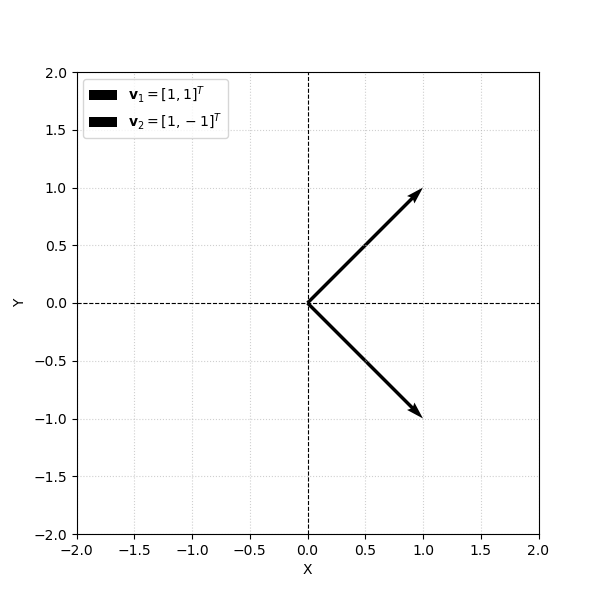
\includegraphics[width=0.60\linewidth]{figs/Eigenvectors.png}
	\makeatletter
    \long\def\@makecaption#1#2{%
      \vskip\abovecaptionskip
      \begin{center}
        #1 #2
      \end{center}
      \vskip\belowcaptionskip}
    \caption{Eigen vectors plotted}
    \label{fig:9}
\end{figure}

\item 


Consider the differential equation:
\begin{align}
\frac{d^2 y}{dx^2} + 2\frac{dy}{dx} + y = 0
\end{align}
with initial conditions $\left.y\right|_{x=0} = 0$ and $\left.\frac{dy}{dx}\right|_{x=0} = 1$. Find the value of the slope $\frac{dy}{dx}$ at $x = \ln\brak{2}$ rounded off to three decimal places.
\hfill (GATE~AE~2026) 

\solution
\begin{enumerate}
\item Theoretical solution
Let $Y(s) = \mathcal{L}\{y\brak{x}\}$. Taking the Laplace transform on both sides:
\begin{align}
\mathcal{L}\left\{\frac{d^2 y}{dx^2}\right\} + 2\mathcal{L}\left\{\frac{dy}{dx}\right\} + \mathcal{L}\{y\} = 0
\end{align}

From equations \eqref{eq:Laplace_1} and \eqref{eq:Laplace_2}:
\begin{align}
\big[s^2 Y(s) - s y\brak{0} - y'\brak{0}\big] + 2\big[s Y(s) - y\brak{0}\big] + Y(s) = 0
\end{align}

Substituting the given initial conditions $y\brak{0} = 0$ and $y'\brak{0} = 1$:
\begin{align}
(s^2 Y(s) - 1) + 2s Y(s) + Y(s) = 0
\end{align}
\begin{align}
(s^2 + 2s + 1) Y(s) = 1
\end{align}
\begin{align}
Y(s) = \frac{1}{(s+1)^2}
\end{align}
Taking the inverse Laplace transform by applying the first frequency shift theorem(\eqref{eq:Laplace_3}) on \eqref{eq:Laplace_4} gives the solution $y\brak{x}$:
\begin{align}
y\brak{x} = x e^{-x}
\end{align}
Differentiating $y\brak{x}$ with respect to $x$:
\begin{align}
\frac{dy}{dx} = \frac{d}{dx}\brak{x e^{-x}} = \brak{1 - x}e^{-x}
\end{align}

Substituting $x = \ln\brak{2}$:
\begin{align}
y'\brak{ln\brak{2}}= \brak{1 - \ln\brak{2}} e^{-\ln\brak{2}}
\end{align}

Since $e^{-\ln\brak{2}} = \frac{1}{2}$:
\begin{align}
= \frac{1 - \ln\brak{2}}{2} \approx \frac{1 - 0.693147}{2} = 0.153426
\end{align}

\item Numerical Solution
Substituting equations \eqref{eq:ED_1} and \eqref{eq:ED_2} into our differential equation, we obtain:
\begin{align}
\frac{y_{n+2} - 2y_{n+1} + y_n}{h^2} + 2 \left( \frac{y_{n+1} - y_n}{h} \right) + y_n = 0
\end{align}
Rearranging, we get:
\begin{align}
y_{n+2} = 2(1 - h)y_{n+1} - (1 - h)^2 y_n
\end{align}
Our initial conditions are:
\begin{align}
y_0=y\brak{0}=0, y_1=y_0+h(y'\brak{0})
\end{align}
Assuming $ln2=0.7$ and $h=0.01$ and evaluating the forward difference at $n=70$, we get:
\begin{align}
	y_{70}'=0.145
\end{align}
\begin{lstlisting}[frame=single, basicstyle=\rmfamily, escapeinside={(*@}{@*)}]
(*@\makebox[\dimexpr\linewidth-2\fboxsep-2\fboxrule\relax][c]{codes/Euler.py}@*)
\end{lstlisting}
\begin{figure}[H]
    \centering
    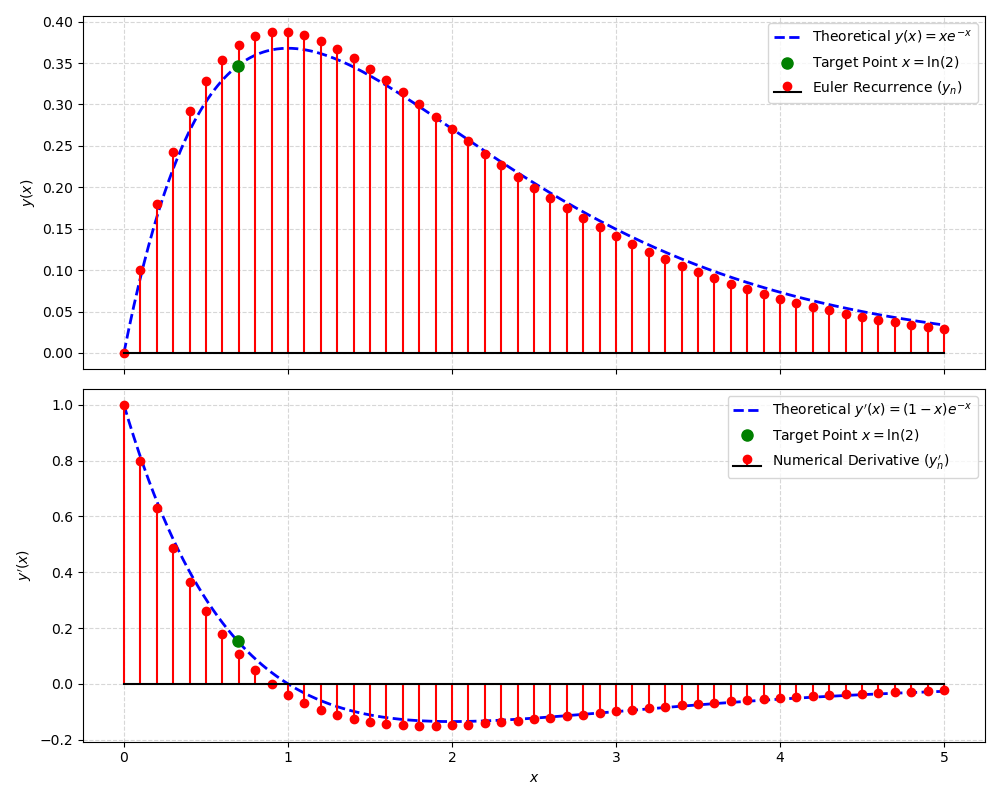
\includegraphics[width=0.75\linewidth]{figs/Euler.png}
	\makeatletter
    \long\def\@makecaption#1#2{%
      \vskip\abovecaptionskip
      \begin{center}
        #1 #2
      \end{center}
      \vskip\belowcaptionskip}
    \makeatother
    \caption{Theoretical Plot vs Plot obtained with Euler's Forward Difference Method}
    \label{fig:13}
\end{figure}
\end{enumerate}

\item 
Find the minimum value of the function $f\brak{x} = \abs{x} + \abs{2x+3}$ for real $x$. \hfill (GATE~AE~2026)

\solution 

The critical points occur where the expressions inside the absolute values equal zero:
\begin{align}
x &= 0 \\[0.5ex]
2x + 3 = 0 &\implies x = -\frac{3}{2} = -1.5
\end{align}

These two critical points divide the real line into three sub-intervals:
\begin{align}
\brak{-\infty, -1.5}, \quad [-1.5, 0), \quad \text{and} \quad [0, \infty)
\end{align}


\begin{itemize}
    \item For $x < -1.5$, bo0th expressions inside the absolute values are negative, so $\abs{x} = -x$ and $\abs{2x+3} = -\brak{2x+3}$:
    \begin{align}
    f\brak{x} = -x - \brak{2x + 3} = -3x - 3
    \end{align}

    \item For $-1.5 \le x < 0$, the term $x$ is negative ($\abs{x} = -x$) while $2x+3$ is non-negative ($\abs{2x+3} = 2x+3$):
    \begin{align}
    f\brak{x} = -x + \brak{2x + 3} = x + 3
    \end{align}

    \item For $x \ge 0$, both expressions are non-negative, so $\abs{x} = x$ and $\abs{2x+3} = 2x+3$:
    \begin{align}
    f\brak{x} = x + \brak{2x + 3} = 3x + 3
    \end{align}
\end{itemize}

Combining these cases gives the complete piecewise definition:
\begin{align}
f\brak{x} = \begin{cases} 
-3x - 3, & \text{if } x < -1.5 \\
x + 3, & \text{if } -1.5 \le x < 0 \\
3x + 3, & \text{if } x \ge 0 
\end{cases}
\end{align}

Analyzing the behavior of each linear segment:
\begin{itemize}
    \item On $\brak{-\infty, -1.5}$, the line $f\brak{x} = -3x - 3$ has a negative slope ($-3$), so $f\brak{x}$ strictly decreases as $x$ approaches $-1.5$.
    \item On $[-1.5, 0)$, the line $f\brak{x} = x + 3$ has a positive slope ($+1$), so $f\brak{x}$ strictly increases as $x$ moves away from $-1.5$.
    \item On $[0, \infty)$, the line $f\brak{x} = 3x + 3$ has a positive slope ($+3$), so $f\brak{x}$ continues to increase.
\end{itemize}

Since $f\brak{x}$ decreases for $x < -1.5$ and increases for $x > -1.5$, the minimum value occurs at $x = -1.5$:
\begin{align}
f\brak{-1.5} = -1.5 + 3 = 1.5
\end{align}
\begin{lstlisting}[frame=single, basicstyle=\rmfamily, escapeinside={(*@}{@*)}]
(*@\makebox[\dimexpr\linewidth-2\fboxsep-2\fboxrule\relax][c]{codes/Modulus\_function.py}@*)
\end{lstlisting}
\begin{figure}[H]
    \centering
    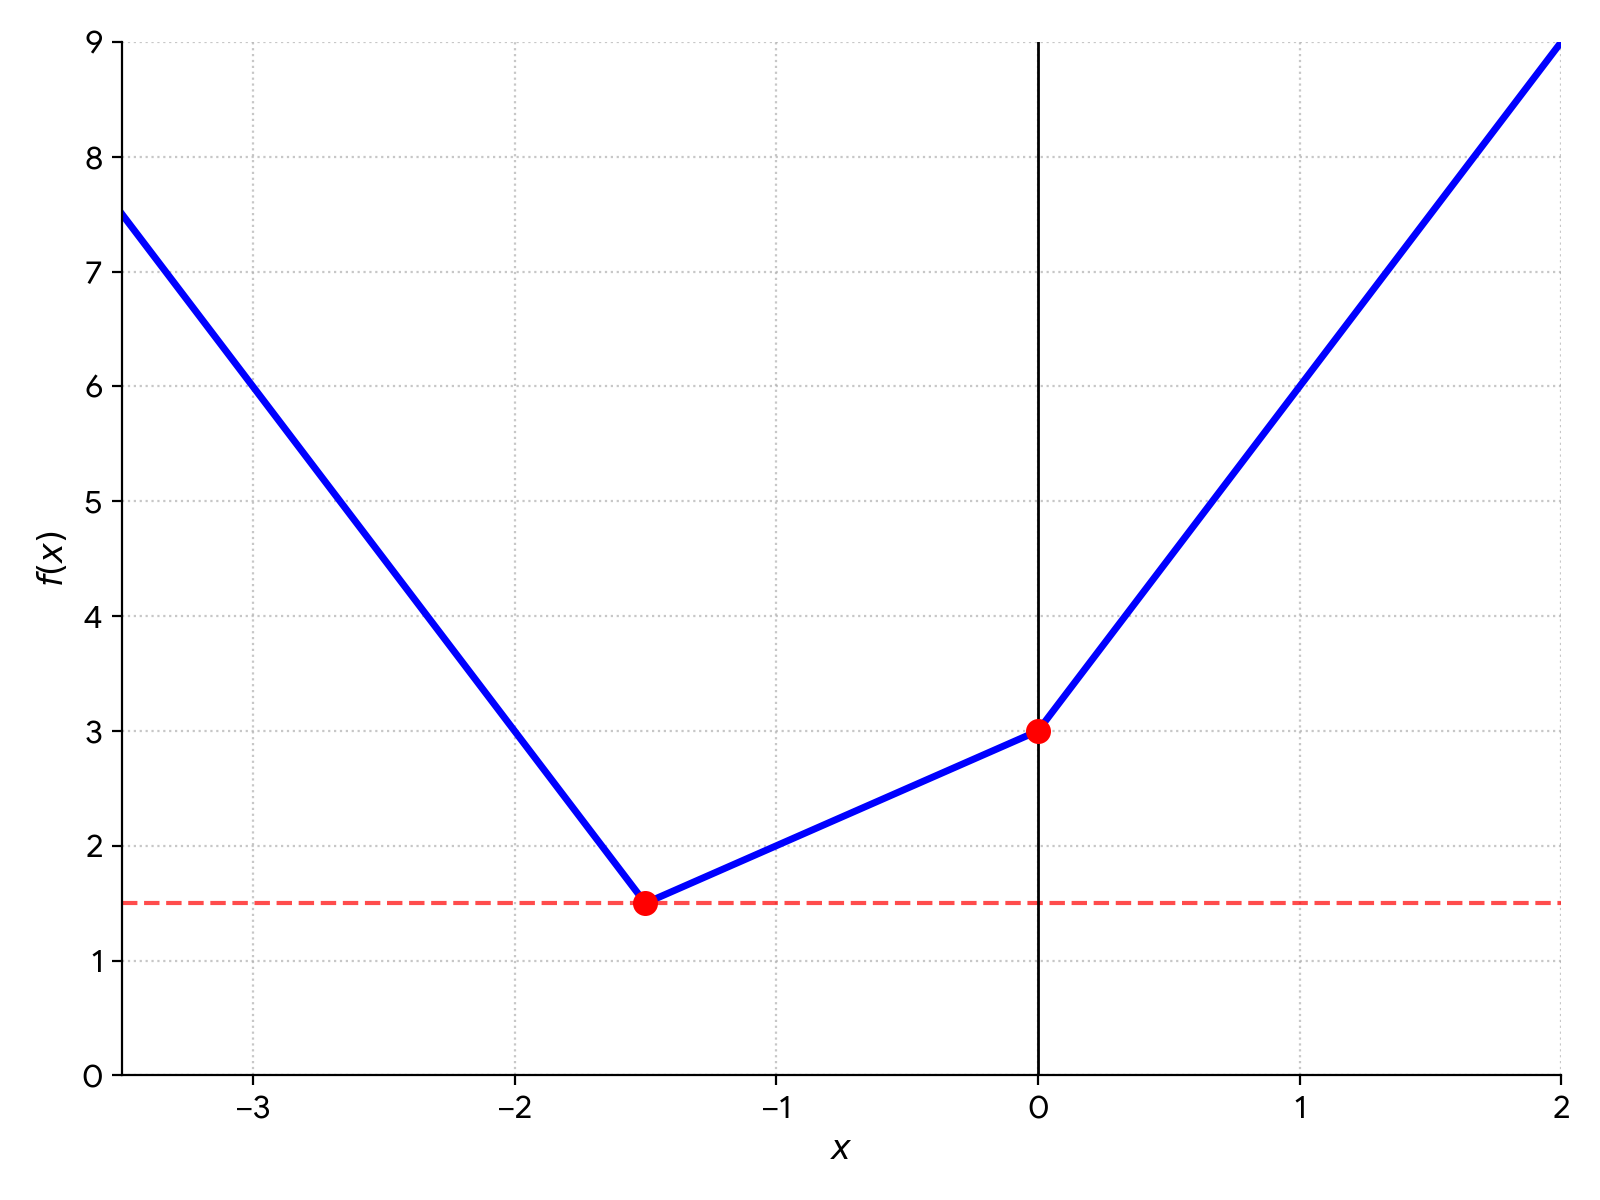
\includegraphics[width=0.75\linewidth]{figs/Modulus_function.png}
	\makeatletter
    \long\def\@makecaption#1#2{%
      \vskip\abovecaptionskip
      \begin{center}
        #1 #2
      \end{center}
      \vskip\belowcaptionskip}
    \makeatother
    \caption{Plot of the function}
    \label{fig:10}
\end{figure}

\item
A bar, spring, and mass system is arranged in series.
\begin{itemize}
    \item Bar: $E = 200\text{ GPa}$, $A = 100\text{ mm}^2$, $L = 100\text{ mm}$
    \item Spring Stiffness: $k = 200\text{ kN/mm}$
    \item Mass: $M = 100\text{ kg}$
\end{itemize}
Find the natural frequency of free vibration $\omega_n$ in $\text{rad/s}$. Also solve the differential equation obtained to obtain the position, velocity and accelaration of the system.
\hfill (GATE~AE~2026)
\begin{figure}[H]
\begin{center}
	\begin{tikzpicture}[scale=1.0, >=Stealth]
    \draw[thick] (-0.2, 4) -- (1.2, 4);

    \draw[thick] (0, 0) rectangle (1, 4);
    \node at (0.5, 2.5) {E, A};

    \draw[thick, <->] (-0.4, 0) -- (-0.4, 4);
    \node[left] at (-0.4, 2) {L};

    \draw[thick, decorate, decoration={zigzag, segment length=3mm, amplitude=2.5mm, pre length=5mm, post length=5mm}] (0.5, 0) -- (0.5, -1.8);
    \node[right=3pt] at (0.7, -0.9) {k};

    \draw[thick] (0.1, -1.8) rectangle (0.9, -2.6);
    \node at (0.5, -2.2) {M};
\end{tikzpicture}


\makeatletter
    \long\def\@makecaption#1#2{%
      \vskip\abovecaptionskip
      \begin{center}
        #1 #2
      \end{center}
      \vskip\belowcaptionskip}
    \makeatother
\caption{Diagram of the system}
\label{fig:11}
\end{center}
\end{figure}

\solution 

The axial stiffness of the uniform bar is:
\begin{align}
k_{\text{bar}} = \frac{AE}{L}
\end{align}
\begin{align}
k_{\text{bar}} = \frac{10^{-4} \times 200 \times 10^9}{0.1} = 2 \times 10^8 \text{ N/m}
\end{align}
With $k = 200 \text{ kN/mm} = 2 \times 10^8 \text{ N/m}$, from \eqref{eq:springs_series}
\begin{align}
k_{\text{eq}} = \frac{k_{\text{bar}} \cdot k}{k_{\text{bar}} + k} = \frac{\brak{2 \times 10^8}\brak{2 \times 10^8}}{2 \times 10^8 + 2 \times 10^8} = 10^8 \text{ N/m}
\end{align}

The natural frequency of free vibration is:
\begin{align}
\omega_n = \sqrt{\frac{k_{\text{eq}}}{M}} = \sqrt{\frac{10^8}{100}} = \sqrt{10^6} = 1000 \text{ rad/s}
\end{align}
Now, to find the position of the system as a function of time, from \eqref{eq:vertical_shm}, we have:
\begin{align}
\frac{d^2 x}{d t^2} = \frac{-k}{M}x = -w_n^2x
\end{align}
Let the initial displacement of the system be $x_0$ and inital velocity be $v_0$. From result \eqref{eq:Laplace_7}, we get:

\begin{align}
x(t) = x_0 \cos(w_nt) + \frac{v_0}{w_n} \sin(w_nt)
\end{align}
Substituting the value of $w_n$, 
\begin{align}
x(t) = x_0 \cos(1000t) + \frac{v_0}{1000} \sin(1000t)
\end{align}
\begin{lstlisting}[frame=single, basicstyle=\rmfamily, escapeinside={(*@}{@*)}]
(*@\makebox[\dimexpr\linewidth-2\fboxsep-2\fboxrule\relax][c]{codes/Spring.py}@*)
\end{lstlisting}
\begin{figure}[H]
    \centering
    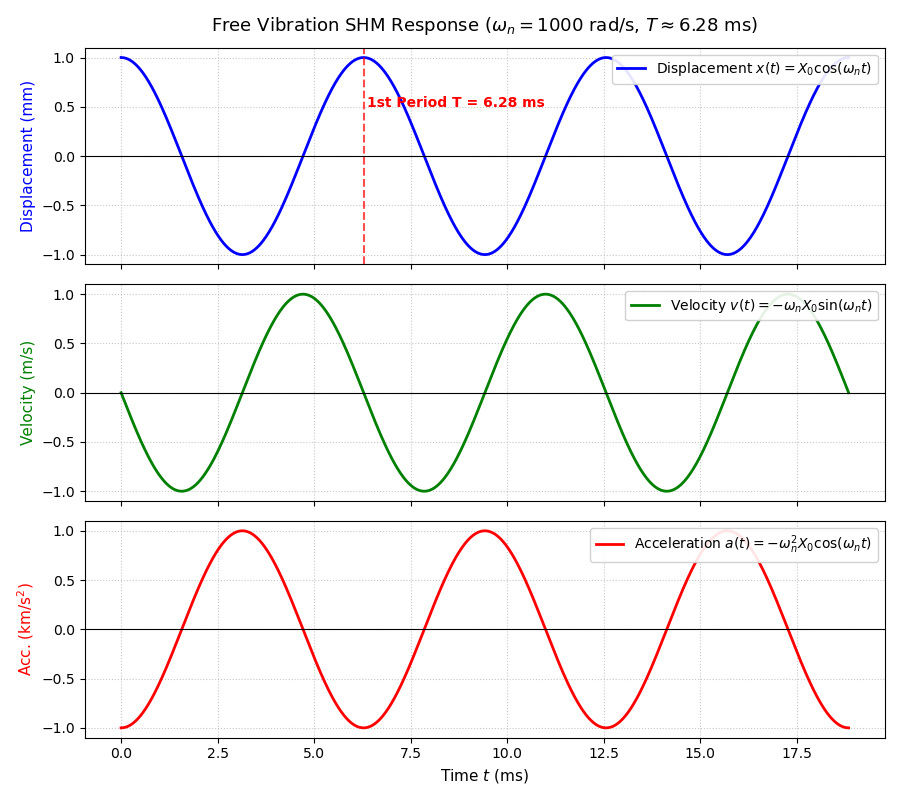
\includegraphics[width=0.65\linewidth]{figs/Spring.png}
    \makeatletter
    \long\def\@makecaption#1#2{%
      \vskip\abovecaptionskip
      \begin{center}
        #1 #2
      \end{center}
      \vskip\belowcaptionskip}
    \makeatother
    \caption{Accelaration, Velocity and Position of the System}
    \label{fig:12}
\end{figure}
\end{enumerate}

